\section{Separation von Amplitude und Phase}
\label{complex:separate}
\rhead{Separation Amplitude / Phase}
\subsection{Warum komplex?}
% TODO: Prof. Müller fragen wegen Notation unendlich-dimensionaler Räume!
Das Problem der Separation von Betrag und Winkel kennt man aus der Fourierteorie mit Cosinus und Sinus.
$a$ und $\omega$ erfüllen ähnliche Zwecke in beiden Welten, die Verschiebung durch $b$ macht für unendlich lange Basisfunktionen aber nur bedingt sinn.
Deshalb kommen bei Fourier nur zwei Familien an Basisfunktionen zum Einsatz, der Cosinus und die um 90\textdegree{} verschobene, orthogonale Version, der Sinus.
Diese beiden Familien an Funktionen bilden eine Hilbertbasis des $L^2(\mathbb{R})$
\[L^2(\mathbb{R}) \cong \mathop{\text{Span}}(\cos\omega t) \times \mathop{\text{Span}}(\sin\omega t) = H_c \times H_s.\]
$H_c$ und $H_s$ sind aufeinander orthogonal und bilden eine Partition des $L^2(\mathbb{R})$.
\[
\forall h_1 \in H_c, h_2 \in H_s: \langle h_1, h_2\rangle = 0
\]
Die Fourier-Transformation berechnet genau die Skalarprodukte mit den Basisfunktionen aus $H_c$ und $H_s$ und folglich die Koordinaten bezüglich $H_c\times H_s$.
\begin{align*}
	\Four : L^2(\mathbb{R}) &\to H_c \times H_s
\end{align*}

Sinus und Cosinus liefern -- in Analogie zu einem Kreis -- kartesischen Koordinaten. 
Für eine Darstellung als Betrag und Winkel sind sie ungeeignet.
Der Trick ist nun, $H_c \times H_s$ durch einen Isomorphismus $\varphi$ mit einem komplexen Hilbertraum zu asoziieren.
\[
	\varphi\colon H_c \times H_s \to \mathbb{C}^\mathbb{R} \colon
	(\cos\omega t,\, \sin\omega t) \mapsto e^{i\omega t}
\]
In einem komplexen Hilbertraum ist die Frage nach Betrag und Winkel direkt beantwortbar.
Die Basisfunktion
\begin{align*}
	z(t) = Ce^{i\omega t} &= |C|e^{i\left(\omega t + \arg C\right)}
\end{align*}
erlaubt durch 
\begin{align*}
	|z(t)| = |C| \quad \text{und}\quad
	\arg z = \arg \omega t + \arg C
\end{align*}
eine separate Betrachtung von Amplitude und Winkel.
Diese Eigenschaft überträgt sich von der Basisfunktion auf den ganzen Raum.

Die Assoziation $\mathbb{R}^\infty  \times \mathbb{R}^\infty \cong \mathbb{C}^\infty$ alleine garantiert die Separierbarkeit von Betrag und Winkel jedoch nicht.
Jedes reelle Wavelet kann kanonisch in $\mathbb{C}^\infty$ eingebettet werden durch
\begin{align*}
	\mathbb{R} \hookrightarrow \mathbb{C}, \quad x \mapsto x.
\end{align*}
Welche Anforderungen müssen also erfüllt sein, damit Betrag und Winkel wirklich voneinander unabhängig sind?
Aufgrund der eulerschen Formel
\begin{equation}
	\cos(x) = \frac{e^{ix} + e^{-ix}}{2}\label{complex:euler}
\end{equation}
kann der Cosinus aus zwei komplexen Exponentialfunktionen mit inverser Frequenz dargestellt werden.
Dies gilt auch, wenn die Amplituden der beiden Exponentialfunktionen nicht übereinstimmen, die Anwesenheit der negativen Frequenz reicht aus, damit ein Teil der Amplitude nicht von der Phase getrennt werden kann.
\begin{align*}
	\frac{e^{i\omega t} + e^{-i\omega t}}{2} &= \cos(\omega t)\\
	\frac{e^{i\omega t} + \Delta e^{-i\omega t}}{2} &=
	\Delta\cos(\omega t) + \frac{1-\Delta}{2} e^{i\omega t}\\
\end{align*}
Ein solches $\Delta$ ``frisst'' uns quasi die erwünschte Exponentialfunktion davon.
Etwas ähnliches geschiet bei positiven, leich unterschiedlichen Frequenzen
\begin{align*}
	\frac{e^{i\omega_1 t} + e^{i\omega_2 t}}{2} &=
	\frac{e^{i(\overline\omega + \Delta \omega) t} + e^{i(\overline\omega-\Delta\omega) t}}{2} \\
	&= e^{i\overline\omega t}\cos(\Delta\omega t)
\end{align*}
Hierbei bezeichnet $\overline\omega=(\omega_1+\omega_2)/2$ die mittlere Frequenz und $\Delta\omega=(\omega_1-\omega_2)/2$ die mittlere Differenz.
Ein $\Delta\omega$ führt also zu einer an- und abschwellenden Exponentialfunktion.
Dies ist für Wavelets verkraftbar, da sie so wie so in der Zeit lokalisiert sind.
$\Delta\omega$ muss nur klein genug sein.

Besitzt ein Wavelet also negative Frequenz-Anteile, dann geht bei diesen Frequenzen die Eigenschaft der Separierbarkeit von Amplitude und Phase verloren.
Zudem sollten die relevanten Frequenzen möglichst kompakt sein.

\subsection{Von Gabor zu Morlet}
\label{complex:gabor-to-morlet}
Durch die Cosinus-Funktion besitzt das Gabor-Wavelet negative Frequenzen, wodurch eine isolierte Betrachtung von Amplitude und Phase unmöglich wird.
Dies möchten wir im Folgenden korrigieren.
Wir wechseln in den Fourierbereich und nutzen aus, dass die Fouriertransformierte einer Gaus-Funktion wieder eine Gaus-Funktion ist,
\[
	\mathcal{F}\left\lbrace e^{-\alpha x^2} \right\rbrace 
	= \frac{1}{\sqrt{2\alpha}}e^{- \frac{\omega^2}{4\alpha}},
\]
und dass die Multiplikation im Zeitbereich zur Faltung im Frequenzbereich wird.
Zudem verwenden wir die Eulerformel~\eqref{complex:euler}.
Die Fouriertransformierte des Gabor-Wavelet wird hierdurch zu

\begin{equation*}
\begin{aligned}
 \hat{\psi}
 & = \mathcal{F}\Bigg\lbrace c_\sigma e^{-\frac{t^2}{2}}\phantom{\Bigg\rbrace}
 \cdot\; \phantom{\mathcal{F}\Bigg\lbrace}
 \Bigg(\cos\left(\sigma t\right) &&
 &&- \kappa_\sigma\Bigg) \Bigg\rbrace \\
 & = \mathcal{F}\Bigg\lbrace c_\sigma e^{-\frac{t^2}{2}} \Bigg\rbrace 
 *\: \mathcal{F}\Bigg\lbrace\Bigg( \frac12 e^{i\sigma t} &+& \frac12 e^{-i\sigma t}
 &&- \kappa_\sigma \Bigg)\Bigg\rbrace\\
 & = \phantom{\mathcal{F}\Bigg\lbrace} c_\sigma e^{- \frac{\omega^2}{2}} \phantom{\Big\rbrace}
 *\:\phantom{\mathcal{F}\Bigg\lbrace} \Bigg(
  \frac{1}{2}\delta(\omega - \sigma) &-&
  \frac{1}{2}\delta(\omega + \sigma) 
 && - \kappa_\sigma\delta(\omega)
  \Bigg).
\end{aligned}
\end{equation*}

Hierbei bezeichnet $\delta(\omega)$ die Dirac-Distribution.
Hieraus lässt sich der negative Anteil des Cosinus leicht entfernen.
Zudem verdoppeln wir den Anteil der positiven Frequenzen (der Grund hierfür erschliesst sich im nächsten Kapitel).
Wir erhalten
\[
	\hat{\psi}^\ast = 
	c_\sigma e^{- \frac{\omega^2}{2}} * \left(
	\delta(\omega - \sigma) +
	\kappa_\sigma\delta(\omega)
	\right),
\]
und durch Rücktransformation in den Zeitbereich
\[
	\psi^\ast = 
	c_\sigma e^{- \frac{t^2}{2}} \cdot \left(
	e^{i\sigma t} +
	\kappa_\sigma
	\right).
\]
Dies ist ein alter Bekannter, das Morlet-Wavelet aus Gleichung~\eqref{cwt:morlet}, dargestellt in Abbildung~\ref{complex:morlet}.
Es eignet sich also besonder gut, um bestimmte Frequenzen in einem Signal zu lokalisieren, allerdings ist es in der Zeit wesentlich schlechter lokalisiert als beispielsweise das Haar-Wavelet.
Dies ist auch in Abbildung~\ref{complex:morlet-ex} ersichtlich, welche die beiden Wavelet-Transformationen unserer Beispiel-Signale zeigt.

\begin{figure}
	\centering
	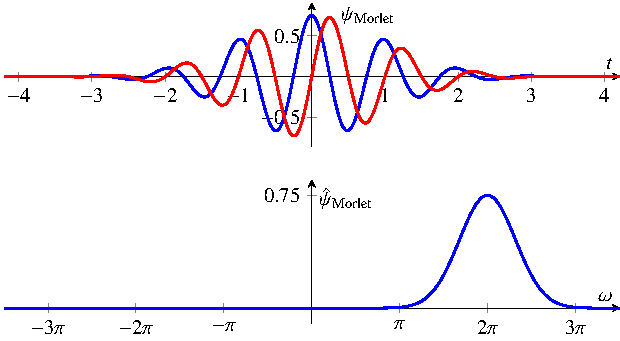
\includegraphics{papers/complex/images/morlet.pdf}
	\caption{Real- (blau) und Imaginärteil (rot) des Morlet-Wavelet für $\sigma = 2\pi$ \label{complex:morlet}}
\end{figure}

\begin{figure}
	\centering
	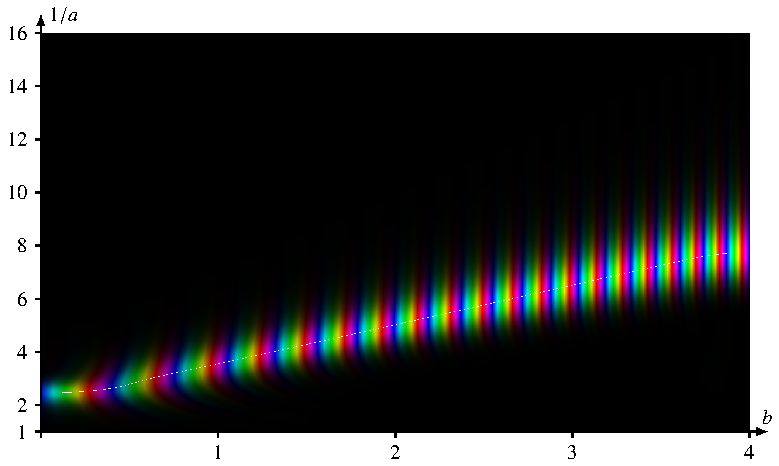
\includegraphics{papers/complex/images/chirp_morlet.pdf}
	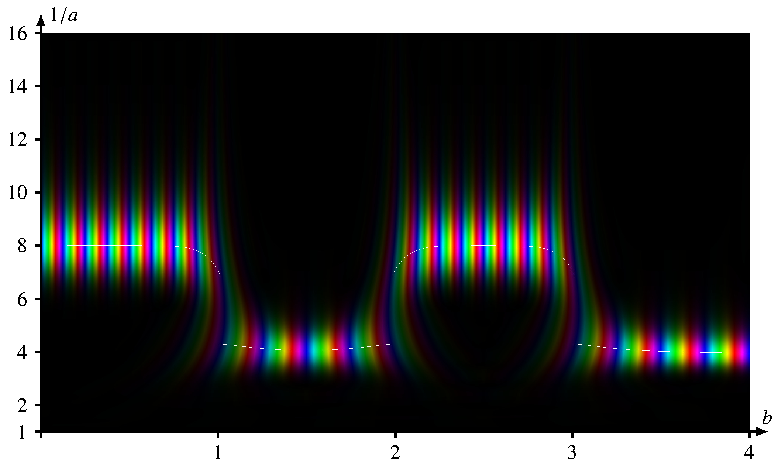
\includegraphics{papers/complex/images/square_morlet.pdf}
	\caption{Farb-codierte Wavelet-Transformationen der beiden Beispielsignale mit dem Morlet-Wavelet.}
	\label{complex:morlet-ex}
\end{figure}
